\chapter{Entwicklung eines Dashboards als moderne Anzeige der Testpoolergebnisse anhand zuvor analysierter bestehender System- und Nutzeranforderungen}
\label{ch:Erstellung Dashboard}
\textcolor{blue}{\textit{einleitende Worte}}\\

% *****************************************************************
\section{Anforderungsanalyse anhand des bestehenden Legacy-Systems und den Nutzerbedürfnissen}
-> potenziell kein Extra Kapitel für IST-Zustand benötigt??

% *****************************************************************
\section{Evaluation und Auswahl des Dashboard-Tools}
\autoref{}

% *****************************************************************
\section{Überblick über den strukturellen Aufbau und Inhalt des Dashboards}
\begin{figure}[H]
    \centering
    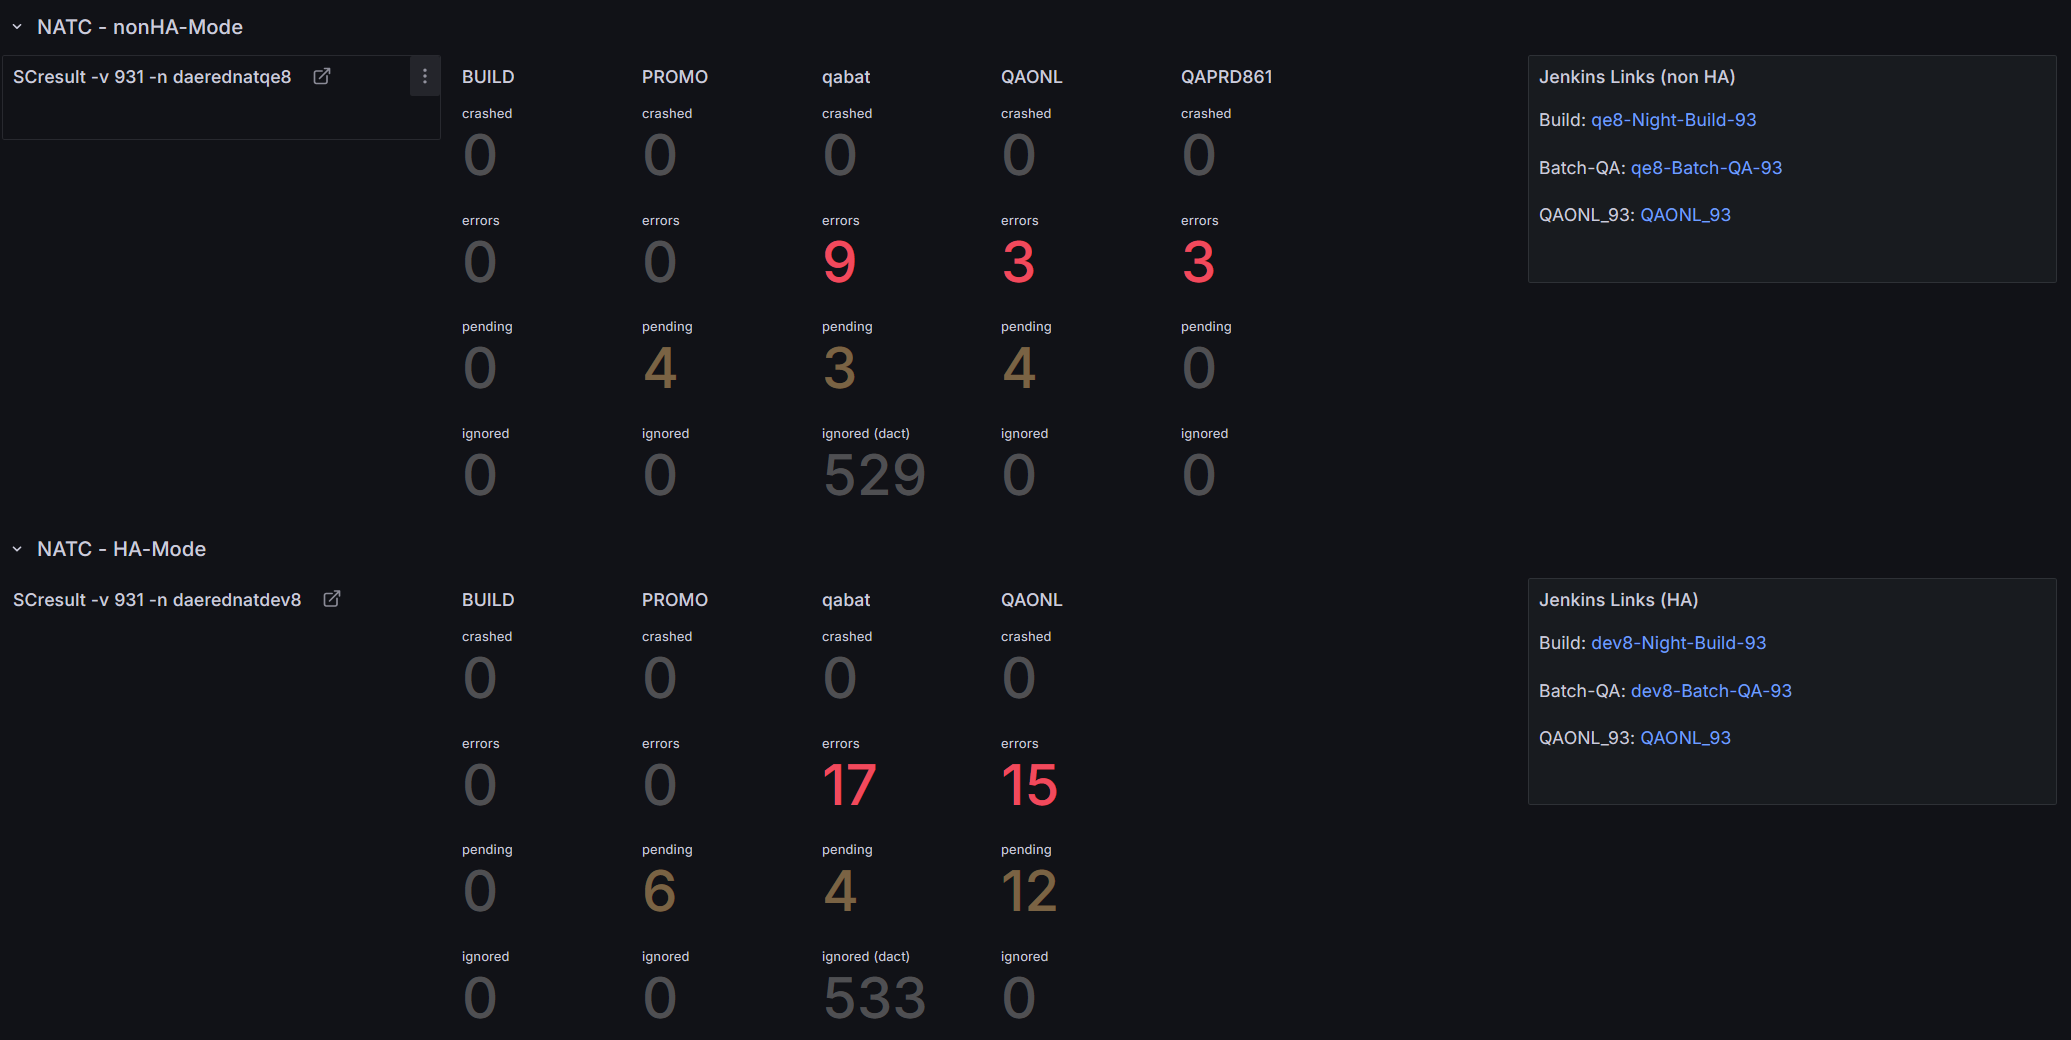
\includegraphics[width=1\linewidth]{Dashboard/20250704_DB_dev.png}
    \caption{Aufbau des gebauten Dashboard \textcolor{red}{(Ersetzen durch zensiertes Bild)}}
    \label{fig:aufbau_dashboard}
\end{figure}

% *****************************************************************
\section{technische Umsetzung des Datenflusses zur Dashboardanzeige}
\begin{figure}[H]
    \centering
    
\includegraphics[width=0.5\linewidth]{Dashboard/Grafana version.png}
    \caption{Grafana-Version}
    \label{fig:grafana_version}
\end{figure}